\chapter{Implementation}

In this chapter what is implemented and what was the problems in the
implementation will be explained.
The implementation has been done in two parts. The first part is the
implementation of the interface in the application, \embtls, and the second part
the implementation of a provider, \tomcrypt, in the interface.

\section{Interface for an application}

The implementation of the interface for the application is, in fact, just a
change of was it was already done.
The function of the interface which was implemented are:
\begin{itemize}[noitemsep]
  \item Hash algorithm
  \item Signature algorithm (Generation and verification)
  \item Message Authentication Code (HMAC)
  \item Cipher algorithm (symmetric, asymmetric, for encryption and decryption)
  \item Random number generator
  \item Diffie Hellman (generation of key pair and calculation of the secret
  key)
  \item Key management
  \item Context management
\end{itemize}

The key pair generator function isn't used in this application, because when the
RSA, DSA or ECDSA are used as key pair exchange, the private key and public key
are in the Certificates.

All parameters in the application which need memory allocation was replaced as
well as possible with context and key management.
For the configuration of each context for any algorithm, all parameters must be
configured, and if a parameter isn't needed, this one must be configured like
``Name\_of\_the\_parameters"\_None.
Before getting an ID of a context and of a key, this ID must be equal to ``-1'',
because some context does different steps depending on the value of the incoming
ID in the interface.


The problems occurred during the implementation of the interface for the
application was:
\begin{itemize}
  \item When sending a Server Key Exchange, the parameters to send are in a
  certain order. In the old implementation, this part was
  done with functions from the provider, but these functions are not
  handled by the new interface. The solution was to rewrite this function
  but directly in the application part and without using the functions from the
  provider. To do that, the sequence to send the parameters should be known,
  which are represented in figure \ref{fig:srv_key_exg}. With the figure \ref{fig:srv_key_exg}
  and the use of the software Wireshark to understand the meaning of what was done in the
  old implementation, it was easier to rewrite this part of the Server Key Exchange.
  This problem and solution is the same for receiving a Server Key Exchange, and
  quick the same for sending and receiving the public key in the Client Key
  Exchange.
  \item When extracting the public key of a certificate, when the
  Certificates are coming from the Server, this part has been done with
  functions from the provider in the old implementation. The functions use
  ASN.1 DER encoding rules \cite{rec:der} function, which are very complex and
  this is not the goal of the project to rewrite this sort of function. That's why another
  source file, named ``gci\_tomcrypt'', has been created to use the function
  from the provider, but with the goal to not have any part of the provider written
  in the application part.
\end{itemize}


\begin{figure}[!ht]
\centering
%\frame{
% trim: left, bottom, right, up
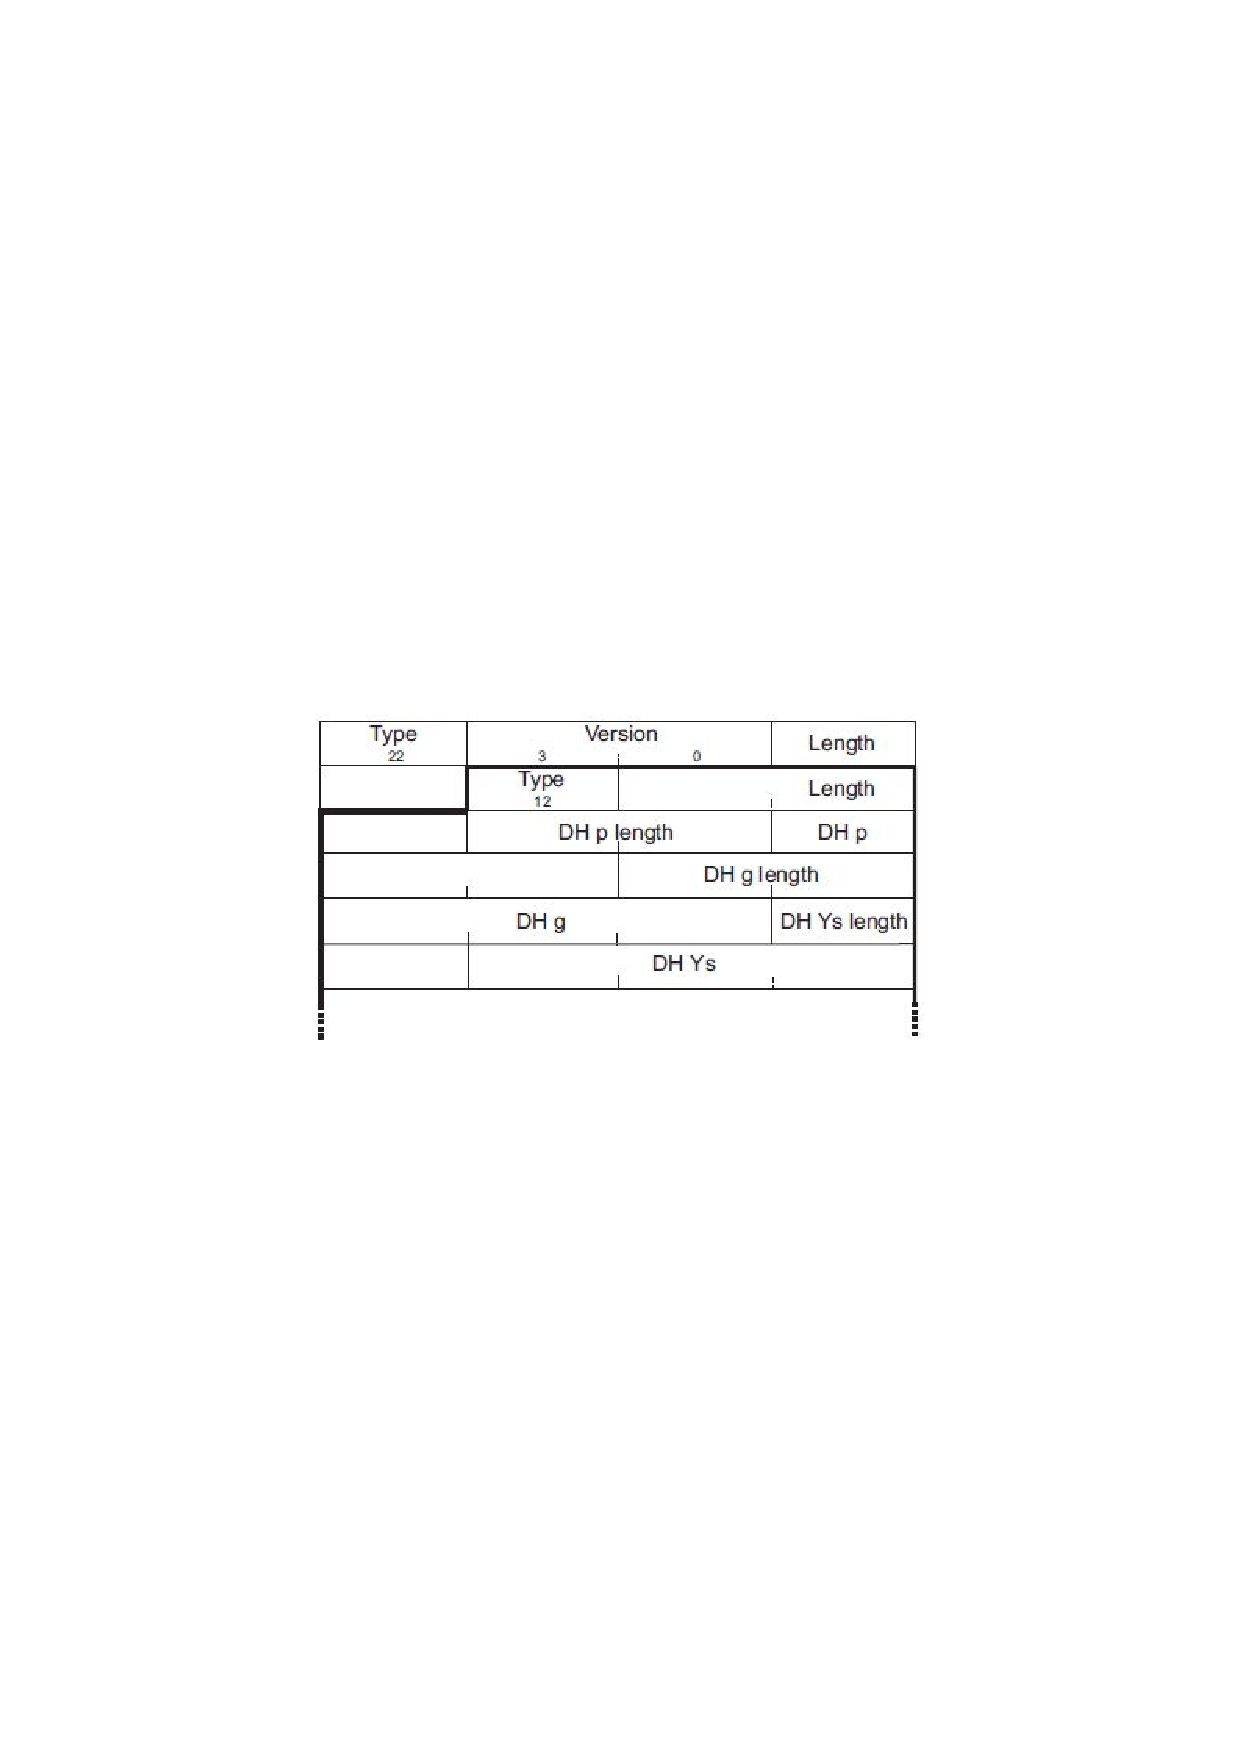
\includegraphics[trim=2cm 12cm 0cm 12cm]{figures/srv_key_exg.pdf}
\caption{Server Key Exchange - Diffie-Hellman as key exchange (source
\cite{book2})}
\label{fig:srv_key_exg}
%}
\end{figure}

\section{Provider for the interface}

The implementation of the \tomcrypt provider to the Generic Cryptographic
Interface (GCI) is important to do all the calculation needed for each algorithm
needed by the application.

For the hash algorithm context (includes the clone of the context of the hash
algorithm), the hash algorithms implemented are:
\begin{itemize}[noitemsep]
  \item MD5 algorithm, which is used by the \embtls application and works
  \item SHA1 algorithm, which is used by the \embtls application and works
  \item SHA224 algorithm, which isn't used by the \embtls application and also
  not tested
  \item SHA256 algorithm, which is used by the \embtls application and works
  \item SHA384 algorithm, which isn't used by the \embtls application and also
  not tested
  \item SHA512 algorithm, which isn't used by the \embtls application and also
  not tested
\end{itemize}

All the hash algorithms have been implemented, but not all have been tested,
because they aren't used by the \embtls application.

For the generation of the signature, the signature/Message Authentication Code
(MAC) algorithms implemented are:
\begin{itemize}[noitemsep]
  \item Hash-based Message Authentication Code (HMAC), which is used
  by the \embtls application and works
  \item RSA algorithm, which is used by the \embtls application and works
\end{itemize}

The signature/Message Authentication Code (MAC) algorithms, which aren't
implemented are:
\begin{itemize}[noitemsep]
  \item Cipher-based Message Authentication Code (CMAC)
  \item DSA
  \item ECDSA
\end{itemize}

These algorithms weren't implemented, because they aren't used by the \embtls
application.

The clone of a signature isn't implemented too, because it's not needed for the
\embtls application


For the verification of the signature, the signature/Message Authentication Code
(MAC) algorithm implemented is the hash-based Message Authentication Code
(HMAC).
The other algorithms (see above, for the generation of a signature) aren't
needed for the \embtls application.


For the generation of key pair (RSA, DSA or ECDSA) none has been implemented,
because none is needed for the \embtls application.

For the cipher (symmetric and asymmetric) algorithms, these implemented are:
\begin{itemize}[noitemsep]
  \item RC4, tested and works
  \item DES, implemented but not tested
  \item 3DES, tested and works
  \item RSA, tested and works
\end{itemize}

The block mode for the symmetric algorithms implemented are:
\begin{itemize}[noitemsep]
  \item CBC
  \item CFB
  \item ECB
  \item GCM
  \item OFB
\end{itemize}
Only the CBC block mode is used by the \embtls application, the others are
implemented, but not tested.

Generation of a Random Number (included the seed) is implemented and works

Diffie-Hellman (and Elliptic Curve of Diffie-Hellman (ECDH)) is implemented and
works.

The context management and key management are implemented and work too.

For the algorithms, which has been implemented but not tested, are implemented,
because the implementation doesn't change a lot compared to this which was
implemented and worked (Hash algorithm and Block mode for the symmetric cipher).

Problems occurred for the implementation of the \tomcrypt provider for the
Generic Cryptographic Interface:

\begin{itemize}
  \item Generation of the signature\newline
  The provider needs, of course, the private key but the public key too to
  generate the signature. In the interface, only one key at a time can be added
  to the context.
  To resolve this problem, first should a context for the
  signature be created, where the configuration of the signature and the private
  key are saved. To begin, the context ID must be initialized to ``-1". This
  context ID will, after the context is created, be greater or equal to ``0".
  Then the function to create the context should be used a second time with the context
  ID previously returned. The public key should be added at this time. The
  interface checks that the context ID is equal to ``-1'', which is not the
  case. Another context won't be created, but the public key will be added to
  the context. The context has, now, the private and public key to generate
  the signature.
  \item When the encryption of the Message Authentication Code (MAC) has to be
  done, depending on the TLS version, if it's greater or equal to TLS 1.1, an
  Initalialization Vector (IV) has to be added to the cipher context before
  encrypting.
  The problem is that, when we arrived at this step, we cannot recreate a cipher
  context with the key needed to encrypt, because this key is, at this step,
  no more available. The only solution is to use the function to create a
  context and to use the context ID returned previously, when the context was
  created with the symmetric key. The context ID is different to ``-1", also a
  new context won't be created, but the new Initialization Vector (IV)
  \cite{wiki:iv} will be added to this context.
\end{itemize}